\documentclass{article}

\usepackage[left=3cm, right=3cm]{geometry}
\usepackage{graphicx}

\graphicspath{{./}}
\pagenumbering{gobble}

\begin{document}

\section*{Normalizing Constant}

Let's say you have a function like $e^{-x^2}$. This is not a valid Probability Density Function (PDF) because it doesn't satisfy the following property: 
\[\int_{-\infty}^{\infty}f(x)dx=1\]
because:

\[\int_{-\infty}^{\infty}e^{-x^2}dx=\sqrt{\pi}\]
Now, how do we get a function that has the same parameters as our original function, like mean and variance, and the densities of the input values, relative to each other, is unchanged? Well, wouldn't dividing $f(x)$ by $\int_{-\infty}^{\infty}f(x)dx$ do it? That is:

\[g(x)=\frac{f(x)}{\int_{-\infty}^{\infty}f(x)dx}\]
In our case:

\[g(x)=\frac{e^{-x^2}}{\sqrt{\pi}}\]
And, obviously:
\[\int_{-\infty}^{\infty}\frac{e^{-x^2}}{\sqrt{\pi}}dx=\frac{1}{\sqrt{\pi}}\int_{-\infty}^{\infty}e^{-x^2}dx=\frac{1}{\sqrt{\pi}}\cdot\sqrt{\pi}=1\]
\\Thus, scaling $f(x)$ with the reciprocal of $\int_{-\infty}^{\infty}f(x)dx$ does the job. Look at the graphs of the function with and without normalization for our example:\\

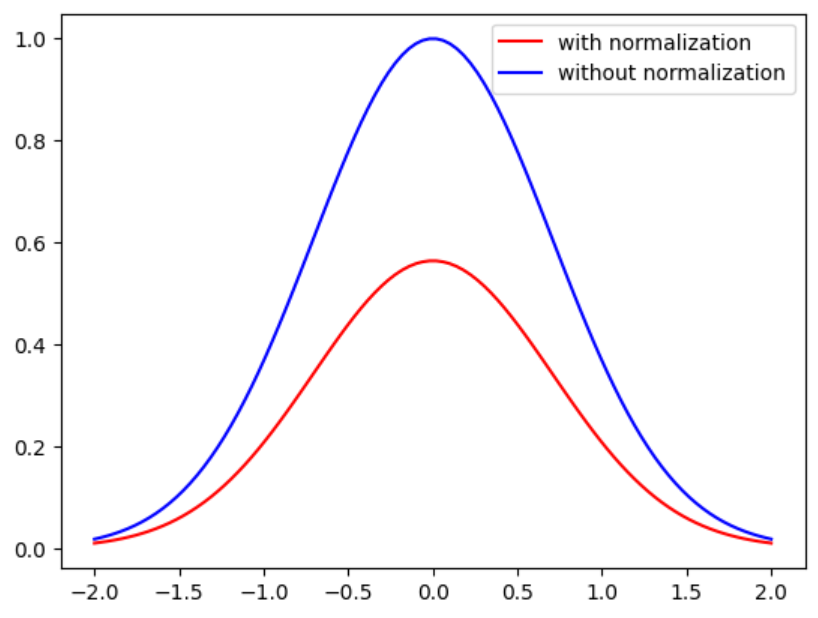
\includegraphics[scale=0.3]{graph}
\centering

\end{document}
